\documentclass{stdlocal}
\begin{document}
\section{Physical Simulations and Monte Carlo Methods} % (fold)
\label{sub:simulation_in_physics_and_mathematics}
  For our purposes, it is enough to explain the application of PRNGs to some given simulation procedures because there is no generic approach on how to randomize an arbitrary physical problem.
  Hence, we will not provide an excessive explanation on the theory of Monte Carlo methods and their application to general physical problems.
  Instead, the focus lies on the understanding of basic concepts and their implementation with respect to well-chosen examples.

  As mentioned in the introduction, the simulation of physical and mathematical systems can be quite time intensive.
  Many degrees of freedom in a resulting partial differential equation makes the problem infeasible to solve deterministically \autocite{landau2014}.
  This is typically called the \enquote{curse of dimensionality} \autocite{mueller2012}.
  As a consequence, we rely on probability theory to estimate the respective solutions and speed-up the simulation.
  Such randomized algorithms are in general called Monte Carlo methods \autocite{mueller2012,landau2014}.

  \begin{definition}[Monte Carlo Method]
    % A Monte Carlo method is an algorithm that uses the realization of random variables, also called random samples, to generate its result.
    A Monte Carlo method is a random variable that computes its result based on given random variables according to an algorithm.
    We call the realization of a Monte Carlo method a run or its execution.
  \end{definition}
  We will not give a rigorous definition of an algorithm but refer to \textcite{hromkovic2011} for detailed information.
  With this definition, the output of an execution of a Monte Carlo method is interpreted as a realization of random variables.
  In contrast to a deterministic algorithm, calling a Monte Carlo method twice with identical input arguments will not necessarily produce the same output again.
  This behavior lets them overcome the curse of dimensionality and as a result they represent an efficient family of generalized algorithms to solve high-dimensional problems.

  To get the idea behind Monte Carlo methods, the observation of direct simulations as given in \textcite{mueller2012} will serve perfectly.
  For some dimension $d\in\setReal$, we want to approximate a value $r\in\setReal^d$ by a Monte Carlo method.
  Direct simulation needs an already existent sequence of iid random variables with their expectation value equal to $r$ which we interpret as random samples.
  But this does not impose strong restrictions because we are mostly able to find such random variables.

  \begin{lemma}[Direct Simulation]
    Let $d\in\setNatural$, $r\in\setReal^d$ and $(X_n)_{n\in\setNatural}$ a sequence of $\setReal^d$-valued iid random variables in $\setIntegrable^2\roundBrackets{\setReal^d,λ}$ with $\expect X_n = r$ for all $n\in\setNatural$.
    In this case, construct the following random variable for all $n\in\setNatural$.
    \[
      D_n \define \frac{1}{n}\sum_{k=1}^n X_k
    \]
    Then for arbitrary sample counts $n\in\setNatural$ the random variable $D_n$ is a Monte Carlo method which fulfills the following equations.
    \[
      \expect D_n = r
      % \separate
      % \var D_n = \frac{\var X_k}{n}
      \separate
      \stddev(D_n) = \frac{\stddev(X_1)}{\sqrt{n}}
      \separate
      \lim_{n\to\infty} \stddev(D_n) = 0
    \]
    % Using the SLLN, we get the following almost everywhere.
    Furthermore, the following limit holds almost everywhere.
    \[
      \lim_{n\to\infty} D_n = r
    \]
  \end{lemma}
  Again, we will give no proof of this lemma and instead refer to \textcite{mueller2012}.
  Please note that the last limit follows from Theorem \ref{theorem:slln} the SLLN.
  The expectation value of the given method is always the result that we wanted to compute.
  This is not a special property.
  But looking at the standard deviation, the error of the direct simulation becomes smaller for a bigger sample count.
  Using a large number of samples will therefore estimate the actual result much more precisely.
  Additionally, the error is decreasing with $\frac{1}{\sqrt{n}}$.
  Hence, the error rate is independent of the given dimension which explains the overcoming of the curse of dimensionality.

  \subsection{Monte Carlo Integration and the Computation of $π$} % (fold)
  \label{sub:monte_carlo_integration_and_the_computation_of_}
    Many simulations involve the calculation of multidimensional integrals.
    As a consequence, the so-called Monte Carlo integration forms the natural application of the direct simulation.
    We want to estimate the integral of a function.
    For given uniformly distributed random variables, we will construct a sequence of random variables such that their expectation value will coincide with the integral.

    \begin{definition}[Monte Carlo Integration]
    \label{definition:monte-carlo-integration}
      Let $d\in\setNatural$ be the dimension, $U\subset\setReal^d$ be a measurable and bounded subset, such that $0 < λ(U) < \infty$, and $f\in\setIntegrable^2(U,λ)$ the function to be integrated.
      Furthermore, let $(X_n)_{n\in\setNatural}$ be a sequence of iid, $U$-valued, and uniformly distributed random variables.
      Then the Monte Carlo integration of $f$ with $n$ samples on the domain $U$ is given by the following expression.
      \[
        \mathrm{MCI}_n(f) \define \frac{λ(U)}{n} \sum_{k=1}^n f\circ X_k
      \]
    \end{definition}
    The domain of definition has to be restricted so that the method has a chance of reducing the overall estimation error.
    Additionally, the function $f$ should be square-integrable such that we are able to get an upper bound on the standard deviation.
    The following lemma will show that Monte Carlo integration is indeed a Monte Carlo method with the properties of a direct simulation.

    \begin{lemma}[Monte Carlo Integration Estimates Value of Integral]
    \label{lemma:monte-carlo-integration}
      Choose the same setting as in the above definition \ref{definition:monte-carlo-integration}.
      In this case for all $n\in\setNatural$, the Monte Carlo integration $\mathrm{MCI}_n(f)$ is a Monte Carlo method and the following statements for the expectation value and standard deviation are fulfilled.
      \[
        \expect \mathrm{MCI}_n(f) = \integral{U}{}{f}{λ}
        \separate
        \stddev\boxBrackets{\mathrm{MCI}_n(f)} \leq \sqrt{\frac{λ(U)}{n} \integral{U}{}{f^2}{λ}}
      \]
    \end{lemma}
    \begin{proof}
      Let $p$ be the probability density of $X_n$.
      Because the random variables are uniformly distributed on $U$, we can express it as follows.
      \[
        \function{p}{U}{[0,\infty)}
        \separate
        p(x) \define \frac{1}{λ(U)}
      \]
      By using substitution and chaining from propositions \ref{proposition:substitution} and \ref{proposition:chaining}, the expectation value can be directly computed.
      \[
        \begin{aligned}[t]
          \expect \mathrm{MCI}_n(f)
          &= \expect \boxBrackets{ \frac{λ(U)}{n} \sum_{k=1}^n f\circ X_k }
          = \frac{λ(U)}{n} \sum_{k=1}^n \expect(f\circ X_k) \\
          &= λ(U) \integral{U}{}{f(x) p(x)}{λ(x)}
          = \integral{U}{}{f}{λ}
        \end{aligned}
      \]
      For the standard deviation, first the variance will be observed.
      Since the sequence of random variables is stochastically independent, the sum can be taken out of the argument.
      Afterwards, we again apply substitution and chaining.
      \[
        \begin{aligned}
          \var \mathrm{MCI}_n(f) &= \var\boxBrackets{ \frac{λ(U)}{n} \sum_{k=1}^n f\circ X_k } = \frac{λ(U)^2}{n^2} \sum_{k=1}^n \var\roundBrackets{f\circ X_k} \\
          &= \frac{λ(U)^2}{n^2} \sum_{k=1}^n \expect\roundBrackets{f\circ X_k}^2 - \boxBrackets{\expect\roundBrackets{f\circ X_k}}^2 \\
          &\leq \frac{λ(U)^2}{n^2} \sum_{k=1}^n \expect\roundBrackets{f\circ X_k}^2 = \frac{λ(U)^2}{n} \integral{U}{}{f^2(x) p(x)}{λ(x)} \\
          &= \frac{λ(U)}{n} \integral{U}{}{f^2}{λ}
        \end{aligned}
      \]
      The inequality is now inferred by the definition of the standard deviation which proofs the lemma.
      \[
        \stddev\boxBrackets{\mathrm{MCI}_n(f)} = \sqrt{\var \mathrm{MCI}_n(f)} \leq \sqrt{\frac{λ(U)}{n} \integral{U}{}{f^2}{λ}}
      \]
    \end{proof}
    In the proof, we basically applied the lemma about the direct simulation.
    So we get the same convergence rate for the expectation value with respect to the standard deviation.
    To get a deeper understanding of this method, consider the estimation of $π$ by Monte Carlo integration.
    For this, we would like to compute the area of a quarter of a circle which is strongly related to π.
    Figure \ref{fig:pi-computation-points} shows the execution of the following process for different realizations.
    \begin{figure}
      \center
      \begin{subfigure}[b]{0.32\linewidth}
        \center
        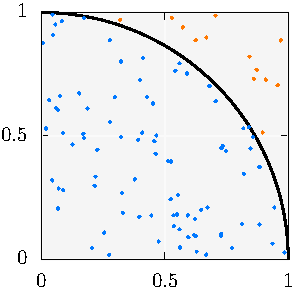
\includegraphics[width=\linewidth]{../../../examples/monte_carlo_pi_100_87.pdf}
        \caption{%
          \quad
          \begin{minipage}[t]{0.5\linewidth}
            $n = 100$ \\
            $s = 87$ \\
            $μ = 3.48$ \\
            $ε \approx 1.07 \cdot 10^{-1}$
          \end{minipage}
        }
      \end{subfigure}
      \hfill
      \begin{subfigure}[b]{0.32\linewidth}
        \center
        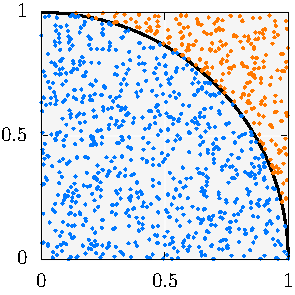
\includegraphics[width=\linewidth]{../../../examples/monte_carlo_pi_1000_765.pdf}
        \caption{%
          \quad
          \begin{minipage}[t]{0.5\linewidth}
            $n = 1000$ \\
            $s = 765$ \\
            $μ = 3.06$ \\
            $ε \approx 2.60 \cdot 10^{-2}$
          \end{minipage}
        }
      \end{subfigure}
      \hfill
      \begin{subfigure}[b]{0.32\linewidth}
        \center
        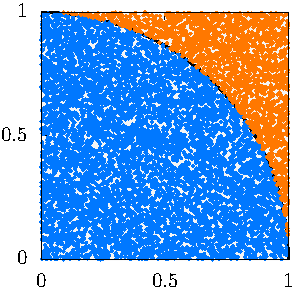
\includegraphics[width=\linewidth]{../../../examples/monte_carlo_pi_10000_7856.pdf}
        \caption{%
          \quad
          \begin{minipage}[t]{0.5\linewidth}
            $n = 10000$ \\
            $s = 7856$ \\
            $μ = 3.1424$ \\
            $ε \approx 2.57 \cdot 10^{-4}$
          \end{minipage}
        }
      \end{subfigure}
      \caption[Monte Carlo Integration and the Computation of π]{%
        The figures show the sample points for different realizations of the Monte Carlo integration $\mathrm{MCI}_n(f)$ for the computation of π.
        Points that lie in the quarter of the unit circle are shown in a blue color whereas other points are shown in orange color.
        The unit circle is represented by a black line.
        The result of the realizations is expressed by the sample mean μ and the relative error with respect to π is expressed by ε.
        The variable $s$ names the count of samples that lie in the unit circle.
      }
      \label{fig:pi-computation-points}
    \end{figure}
    Computing the area of a subset is in general done by integration.
    Therefore we choose $d=2$ and $U\define [0,1]^2$ with $λ(U) = 1$.
    Thus, the random variable $X_n$ will be uniformly distributed on $[0,1]^2$ for all $n\in\setNatural$.
    The last part consists of the construction of the function $f$.
    First, define the set which characterizes the quarter of the unit circle.
    \[
      G \define \set{x \in [0,1]^2}{\norm{x} \leq 1}
      \separate
      λ(G) = \frac{π}{4}
    \]
    Based on this set, the function $f$ can be expressed through the use of the characteristic function of $G$ and by scaling its value.
    \[
      f \define 4\cdot\mathds{1}_G
      \separate
      \integral{U}{}{f}{λ} = 4 \integral{[0,1]^2}{}{\mathds{1}_G}{λ} = 4\cdotλ(G) = π
    \]
    Simulating the integral of $f$ will therefore give us an estimation of π.
    For a more detailed analysis, we will also compute the exact standard deviation of this Monte Carlo integration by using the above lemma \ref{lemma:monte-carlo-integration}.
    \[
      \integral{U}{}{f^2}{λ} = 16 \integral{[0,1]^2}{}{\mathds{1}_G}{λ} = 16\cdot λ(G) = 4π
    \]
    \[
      \begin{aligned}
        \var\roundBrackets{f\circ X_1}
        &= \expect\roundBrackets{f\circ X_1}^2 - \boxBrackets{\expect\roundBrackets{f\circ X_1}}^2
        = \integral{U}{}{f^2}{λ} - \roundBrackets{\integral{U}{}{f}{λ}}^2 \\
        &= 4π - π^2 = π(4-π)
      \end{aligned}
    \]
    \[
      \stddev\roundBrackets{\mathrm{MCI}_n(f)} = \sqrt{\frac{π(4-π)}{n}} \leq 2\sqrt{\frac{π}{n}}
    \]
    In figure \ref{fig:pi-computation-plots}, we can see this behavior for some actual simulations.
    By taking a larger amount of samples, the volume of the quarter of the unit circle becomes more occupied as can be seen in figure \ref{fig:pi-computation-points}.
    As a consequence, the estimation of π will be more precise.
    Furthermore, figure \ref{fig:pi-computation-plots} shows that the error of the estimation can also be estimated and will be more precise for a larger sample count.
    \begin{figure}
      \center
      \begin{subfigure}[b]{0.49\linewidth}
        \center
        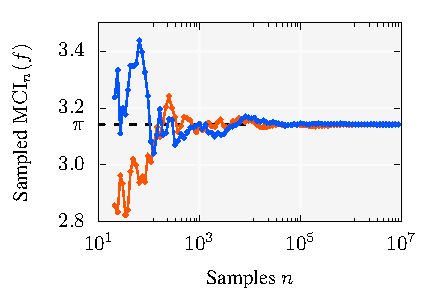
\includegraphics[width=\linewidth]{../../../examples/monte_carlo_pi_plot.pdf}
      \end{subfigure}
      \begin{subfigure}[b]{0.49\linewidth}
        \center
        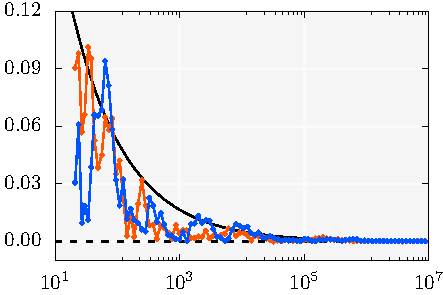
\includegraphics[width=\linewidth]{../../../examples/monte_carlo_pi_plot_error.pdf}
      \end{subfigure}
      \caption[Monte Carlo Integration Plots for the Computation of π]{%
        Each of the diagrams shows two different versions, colored in orange and blue, of realizations of the Monte Carlo integration $\mathrm{MCI}_n(f)$ for the computation of π for different values of $n$.
        The left one displays the estimated value of π and the right one displays its relative error with respect to π.
        Hereby the black line shows the exact relative standard deviation with respect to π of the Monte Carlo integration.
      }
      \label{fig:pi-computation-plots}
    \end{figure}

    Later, we will use the computation of π as benchmark routine to measure the performance of PRNGs with respect to different aspects of their implementation.
    In these cases, the error of π should be in some given range
    Assume we want to use $10^8$ samples to estimate the value of π.
    According to the formula above for the standard deviation, we get an error of approximately $0,00016$ which means we should at least get a precision of four digits, such that π should approach the value $3.1415$ with a varying last digit.

    To use the described Monte Carlo integration for estimating π, an actual implementation in C++ is needed.
    The following code snippet provides the basic algorithm relying on the random utilities given by the standard template library (STL) of the C++ programming language.
    Because C++ is a strongly typed language which is working with templates for type abstraction, the given code uses templates to generalize the usage of different RNG types, as well as different real and integer number types.
    Typically, we will use the \code{float} type as the real number type and the \code{int} type as the integer type.

    \inputCodeBlock[title=monte\_carlo\_pi.hpp]{code/monte_carlo_pi.hpp}
    The implementation of the algorithm does not introduce any irregularities and can directly be deduced from the mathematical formulation.
    First, we define the standard uniform distribution for the RNG and an integer number \code{samples\_in\_circle} as zero which will be used to count the number of samples that lie inside the unit circle.
    In the following \code{for} loop every run will construct two uniformly distributed random numbers which together will define the position of random two-dimensional point in the unit square.
    We then evaluate the circle condition adding it to \code{samples\_in\_circle} resulting in an incrementation by one if it is true and zero otherwise.
    At the end, the code computes the correct result by calculating the division and scaling the output.

    % The application of the given library function is shown in the following source file.
    % \inputCodeBlock[title=monte\_carlo\_pi.cpp]{code/monte_carlo_pi.cpp}

    The computation of π is only an academic example that should not be used in reality because there are much more efficient ways to estimate it.
    But as we will see, it is perfectly suited as a benchmark to test different kinds of RNGs because the main part of the algorithm consists of generating a lot of random numbers while using their values to actually compute a result.
    Evaluating the circle condition for generated random numbers is fast and will not introduce a lot of bias in the actual measurement.
    Besides, it is the most simplest example of a non-trivial Monte Carlo integration.
    A lot of physical problems rely on Monte Carlo integration.
    In the end, all these problems can be broken down into similar form as the computation of π.
  % subsection monte_carlo_integration_and_the_computation_of_ (end)

  \subsection{Metropolis-Hastings Algorithm and the Ising Model} % (fold)
  \label{sub:metropolis_hastings_algorithm_and_the_ising_model}

  % subsection metropolis_hastings_algorithm_and_the_ising_model (end)

  \subsection{Photon Propagation and Physically Based Rendering} % (fold)
  \label{sub:photon_propagation_and_physically_based_rendering}
    In computer graphics, the rendering of realistic images based on physical principles requires the simulation of global illumination effects.
    Global illumination is formally described by the so-called rendering equation, also known as light transport equation (LTE).
    There exist several different formulations of the LTE, such as the surface form and the path integral formulation, which are all equivalent and are used to derive advanced methods to actually estimate the light distribution in space consisting of differing objects.
    The LTE can be derived by applying principles of geometric optics to the law of the conservation of energy for electromagnetic radiation.
    A detailed explanation is given in \textcite{pharr2016} and a mathematically rigorous discussion can be read in \textcite{pawellek2017}.

    Typically, the LTE cannot be evaluated analytically for complex geometries.
    As a consequence, there are multiple famous simulation strategies, like path tracing, bidirectional path tracing, metropolis light transport, and photon mapping, to approximate its solutions.
    All of these strategies have in common that they are somehow estimating the light distribution in space through Monte Carlo methods.
    Because of the integral appearing inside the equation, all algorithms make great use of Monte Carlo integration in different ways.
    Path tracing, for example, is using the path integral formulation of the LTE by importance sampling different paths of light through the scene starting from the observer and ending at a light source.
    At every vertex of the path, Russian roulette decides if the ray has to be reflected, transmitted or absorbed.
    In general, the algorithm has to compute several hundreds of sample paths for every pixel on the screen to reduce the noise and get an acceptable estimation  of the actual light distribution.
    As a consequence, the tracing of rays and the propagation of photons through a scene needs to use a really large amount of random numbers.

    The tracing of light rays is strongly connected to photon propagation in space.
    From an abstract point of view, we can think of light rays as single photons or packets of photons.
    Light rays are used to gather the radiance arriving at the observer whereas photons propagate flux from a light source.
    Both of them adhere to the same laws even if they are interpreted differently.
    Hence, photon tracing works exactly the same way as ray tracing.
    A usual application of this phenomenon is the photon mapping algorithm.
    The movement and transmission of differing photons or rays does not depend on each other.
    Due to the high amount of random numbers needed and the large degree of independence the simulation of global illumination by using Monte Carlo methods is a perfect candidate to measure the performance improvement by applying vectorized PRNGs.
    This claim is even supported by an already existing strong usage of SIMD instructions for the current most efficient ray and path tracing engines \autocite{embree}.

    In this thesis, it is not possible to provide a complete ray tracing framework to test the application of vectorized PRNGs.
    But we are able to construct a simplified version which is using the developed PRNGs to simulate the propagation of photons.
    This smaller simulation focuses on the most important physical effects and ignores subtleties that would introduce bias in the performance measurements.
    We will provide the physical background concerning photon propagation.

    \subsubsection*{Surface Interaction} % (fold)
    \label{ssub:surface_interaction}

    % subsubsection surface_interaction (end)

    \subsubsection*{Volume Scattering} % (fold)
    \label{ssub:volume_scattering}

    % subsubsection volume_scattering (end)
  % subsection photon_propagation_and_physically_based_rendering (end)
% section simulation_in_physics_and_mathematics (end)
\end{document}